\documentclass[9pt]{revtex4-1}
\usepackage{graphicx}
\title{Lista de galaxias candidatas -- DR1}

\begin{document}
\maketitle

\begin{@twocolumnfalse}
\section{DR1}

\begin{center}
\begin{tabular}{ l c c }
Nombre & Tipo & Redshift (z) \\
\hline
\hline \\
UGC00312 & G & 0.014507 -- 0.014557 \\
UGC07012 & G & 0.010277 \\
UGC08733 & G & 0.007799 \\
UGC09476 & Ggroup -- G & 0.010881 \\
NGC7819 & G -- Ggroup & 0.016538 -- 0.017299 \\
NGC0477 & G (SN2002jy) & 0.019600 \\
NGC2916 & G *(Revisar con Jaime) & *Revisar con Jaime \\
NGC7321 & G (SN2013di SN2008gj)) & 0.023833 \\
IC1256  & G & 0.015778 \\
NGC0036 & G & 0.020114 \\
NGC0776 & G (SN1999di) & 0.016415 \\
NGC4210 & G (SN2002ho) & 0.009113 \\
NGC4185 & G (SN1982C)  & 0.013022 \\
IC0776  & G & 0.008232 \\
NGC5000 & G (SN2003el) & 0.018706 \\
UGC08781 & G & 0.025324 \\
NGC5406 & G (SN1977B) & 0.017352
\end{tabular}
\end{center}

\end{@twocolumnfalse}

%\twocolumngrid
%\appendix

%\onecolumngrid
%\appendix

%\clearpage

\twocolumngrid
\begin{figure}
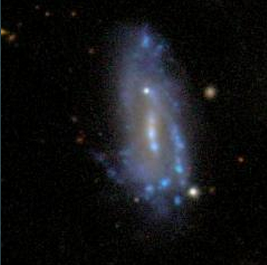
\includegraphics[scale=0.3]{UGC00312.png}
\caption{UGC00312}
\end{figure}
\begin{figure}
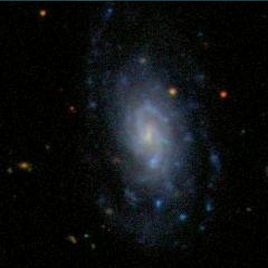
\includegraphics[scale=0.3]{UGC07012.png}
\caption{UGC07012}
\end{figure}
\begin{figure}
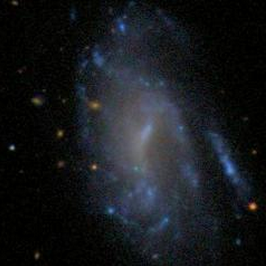
\includegraphics[scale=0.3]{UGC08733.png}
\caption{UGC08733}
\end{figure}
\begin{figure}
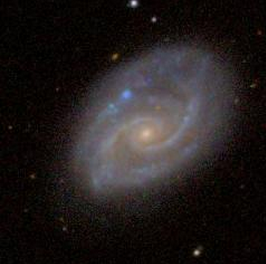
\includegraphics[scale=0.3]{UGC09476.png}
\caption{UGC09476}
\end{figure}
\begin{figure}
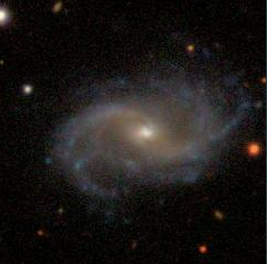
\includegraphics[scale=0.3]{NGC7819.png}
\caption{NGC7819}
\end{figure}




\begin{figure}
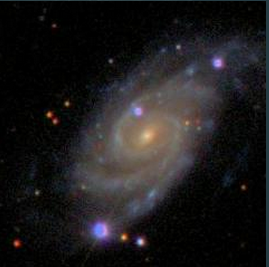
\includegraphics[scale=0.3]{NGC0477.png}
\caption{NGC0477}
\end{figure}
\begin{figure}
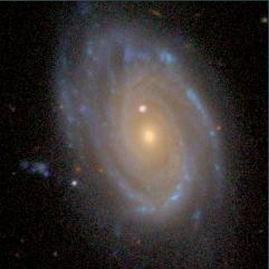
\includegraphics[scale=0.3]{NGC2916.png}
\caption{NGC2916}
\end{figure}
\begin{figure}
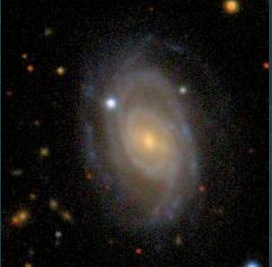
\includegraphics[scale=0.3]{NGC7321.png}
\caption{NGC7321}
\end{figure}
\begin{figure}
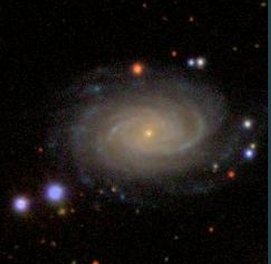
\includegraphics[scale=0.3]{IC1256.png}
\caption{IC1256}
\end{figure}
\begin{figure}
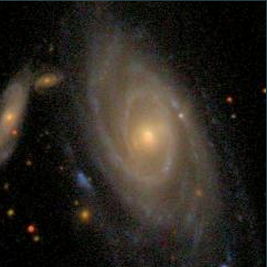
\includegraphics[scale=0.3]{NGC0036.png}
\caption{NGC0036}
\end{figure}



\begin{figure}
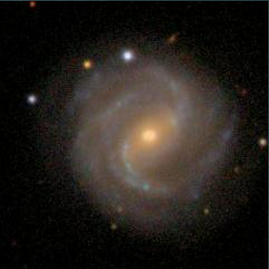
\includegraphics[scale=0.3]{NGC0776.png}
\caption{NGC0776}
\end{figure}
\begin{figure}
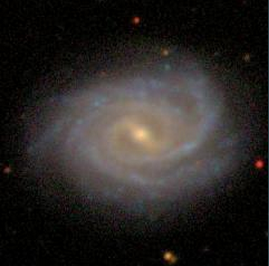
\includegraphics[scale=0.3]{NGC4210.png}
\caption{NGC4210}
\end{figure}
\begin{figure}
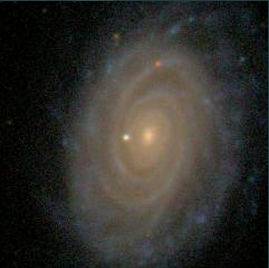
\includegraphics[scale=0.3]{NGC4185.png}
\caption{NGC4185}
\end{figure}
\begin{figure}
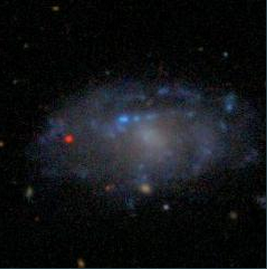
\includegraphics[scale=0.3]{IC0776.png}
\caption{IC0776}
\end{figure}
\begin{figure}
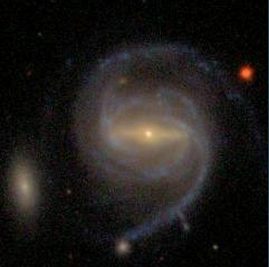
\includegraphics[scale=0.3]{NGC5000.png}
\caption{NGC5000}
\end{figure}



\begin{figure}                                           
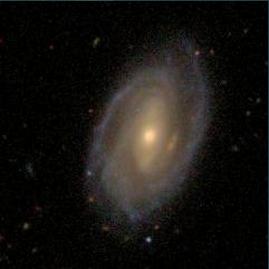
\includegraphics[scale=0.3]{UGC08781.png}
\caption{UGC08781}
\end{figure}
\begin{figure}
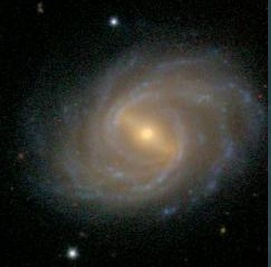
\includegraphics[scale=0.3]{NGC5406.png}
\caption{NGC5406}
\end{figure}

\clearpage

\begin{@twocolumnfalse}

\onecolumngrid

\section{DR2}
 \begin{center}
 \begin{tabular}{ l c c }
 
 Nombre & Tipo & Redshift (z) \\
 \hline
 \hline \\
 
 
 NGC7819 & G -- Ggroup & 0.016538 -- 0.017299 \\ %ya
 NGC0001 & G & 0.015177 \\ %ya
 NGC0036 & G & 0.020114 \\ %ya
 UGC00312(NOTES01) & G & 0.014557 -- 0.014507 \\ %ya
 NGC0171 & G & 0.013043 \\ %ya
 NGC0180 & G (SN2001dj) & 0.017616 \\ %ya
 NGC0237 & G & 0.013926 \\ %ya
 NGC0496 & G & 0.020034 \\ %ya
 NGC0776 & G (SN1999di) & 0.016415 \\ %ya
 NGC2253 & G & 0.011885 \\ %ya
 NGC2347 & G (SN2001ee) & 0.014747 \\ %ya
 NGC2730 & G & 0.012782 \\ %ya
 NGC2916 & *preguntar & *preguntar \\ %ya
 NGC3381 & G & 0.005434 \\ %ya
 NGC3614 & *preguntar & *preguntar \\ %ya
 NGC3811 & G (SN1971K SN1969C) & 0.010357 \\ %ya
 UGC07012 & G & 0.010277 \\ %ya
 NGC4185 & G (SN1982C) & 0.013022 \\ %ya
 NGC4210 & G (SN2002ho) & 0.009113 \\ %ya
 IC0776  & G & 0.008232 \\ %ya
 NGC4470 (CXO J122937.8+074931) & G -- XrayS & 0.007809 \\ %ya
 NGC5000 & G (SN2003el) & 0.018706 \\ %ya
 NGC5205 & G & 0.005891 \\ %ya
 UGC08733 & G & 0.007799 \\ %ya
 UGC08781 *dudas & G & 0.025324 \\ %ya
 NGC5378 & G (SN1991ak) & 0.010147 \\ %ya
 NGC5406 & G (SN1977B) & 0.017352 \\ %ya
 UGC09067 & G & 0.026151 \\ %ya
 % REVISAR -----------------------------------------------------------
 NGC0036 & G & 0.020114 \\ %ya
 NGC0776 & G (SN1999di) & 0.016415 \\ %ya
 NGC4210 & G (SN2002ho) & 0.009113 \\ %ya
 NGC4185 & G (SN1982C)  & 0.013022 \\ %ya
 IC0776  & G & 0.008232 \\ %ya
 NGC5000 & G (SN2003el) & 0.018706 \\ %ya
 UGC08781 & G & 0.025324 \\ %ya
 NGC5406 & G (SN1977B) & 0.017352 \\ %ya
 %REVISAR ------------------------------------------------------------
 NGC5520 & G & 0.006261 \\ %ya
 NGC5614 & G & 0.012982 \\ %ya
 NGC5630 & G (SN2005dp 2006am) & 0.008856 \\ %ya
 NGC5720 & G & 0.025985 \\ %ya
 UGC09476 & Ggroup -- G & 0.010881 \\ %ya
 NGC5888 & G (SN2010fv SN 2007Q) & 0.029123 \\ %ya
 IC4566 & G & 0.019260 \\ %ya
 NGC6004 & G & 0.012762 \\ %ya
 NGC6063 & G (SN1999ac) & 0.009500 \\ %ya
 NGC6154 & G & 0.020064 \\ %ya
 
 \end{tabular}
 \end{center}
 
 \begin{center}
 \begin{tabular}{ l c c }
 Nombre & Tipo & Redshift(z)\\
 \hline 
 \hline \\
 
 IC1256 & G & 0.015778 \\ %ya
 NGC6941 & G & 0.020761 \\ %ya
 UGC11649 & G & 0.012669 \\ %ya
 NGC7321 & G (SN2013di SN2008gj) & 0.023833 \\ %ya
 UGC12224 & G & 0.011695 \\ %ya
 NGC7489 & G & 0.020811 \\ %ya
 NGC7625 *dudas & G & 0.005447 \\ %ya
 NGC7653 & G & 0.014227 \\ %ya
 NGC7716 & GGroup -- G & 0.009700 -- 0.008604 \\ %ya
 NGC5947 & G & 0.019650 \\  %YA
 
 \end{tabular}
 \end{center}
 
\end{@twocolumnfalse}
 
%\clearpage

\twocolumngrid

\begin{figure}
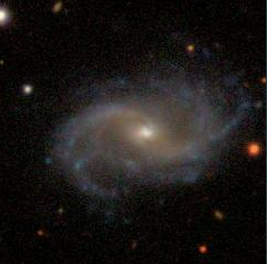
\includegraphics[scale=0.3]{NGC7819.png}
\caption{NGC7819}
\end{figure}
\begin{figure}
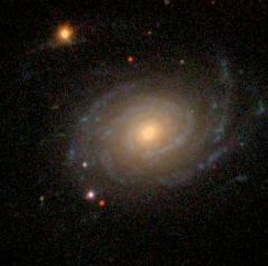
\includegraphics[scale=0.3]{NGC0001.png}
\caption{NGC0001}
\end{figure}
\begin{figure}
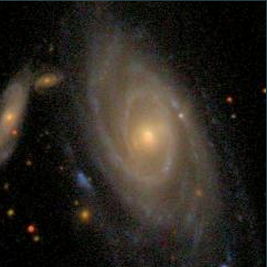
\includegraphics[scale=0.3]{NGC0036.png}
\caption{NGC0036}
\end{figure}
\begin{figure}
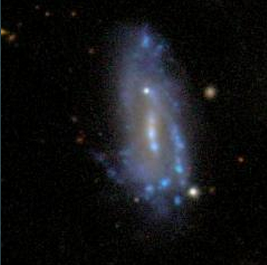
\includegraphics[scale=0.3]{UGC00312.png}
\caption{UGC00312}
\end{figure}
\begin{figure}
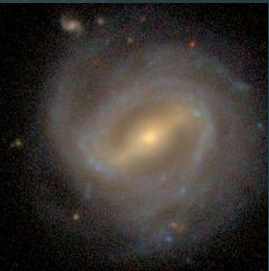
\includegraphics[scale=0.3]{NGC0171.png}
\caption{NGC0171}
\end{figure}
\begin{figure}
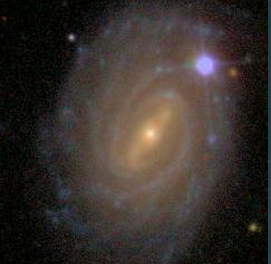
\includegraphics[scale=0.3]{NGC0180.png}
\caption{NGC0180}
\end{figure}

%\clearpage

\begin{figure}
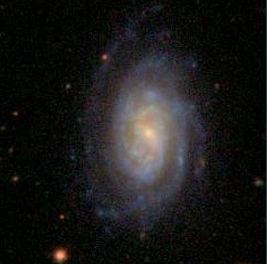
\includegraphics[scale=0.3]{NGC0237.png}
\caption{NGC0237}
\end{figure}
\begin{figure}
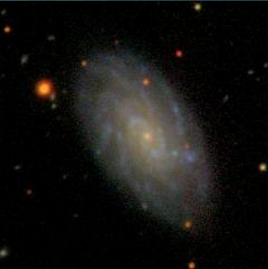
\includegraphics[scale=0.3]{NGC0496.png}
\caption{NGC0496}
\end{figure}
\begin{figure}
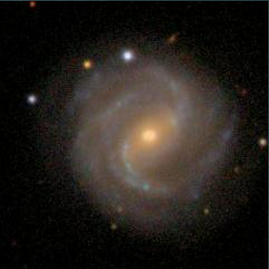
\includegraphics[scale=0.3]{NGC0776.png}
\caption{NGC0776}
\end{figure}
\begin{figure}
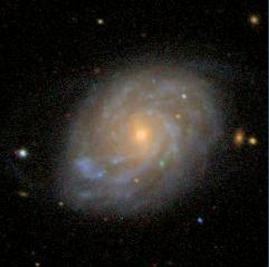
\includegraphics[scale=0.3]{NGC2253.png}
\caption{NGC2253}
\end{figure}
\begin{figure}
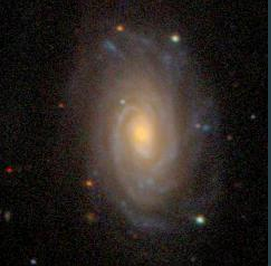
\includegraphics[scale=0.3]{NGC2347.png}
\caption{NGC2347}
\end{figure}

\clearpage

\begin{figure}
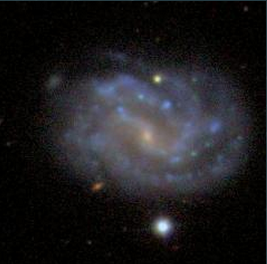
\includegraphics[scale=0.3]{NGC2730.png}
\caption{NGC2730}
\end{figure}
\begin{figure}
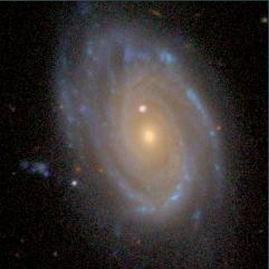
\includegraphics[scale=0.3]{NGC2916.png}
\caption{NGC2916}
\end{figure}
\begin{figure}
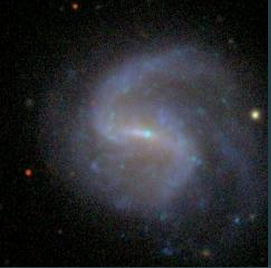
\includegraphics[scale=0.3]{NGC3381.png}
\caption{NGC3381}
\end{figure}
\begin{figure}
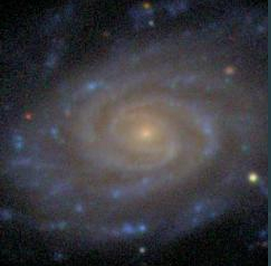
\includegraphics[scale=0.3]{NGC3614.png}
\caption{NGC3614}
\end{figure}
\begin{figure}
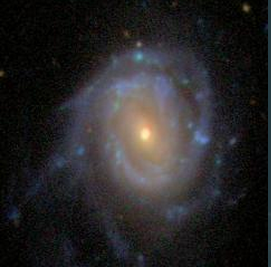
\includegraphics[scale=0.3]{NGC3811.png}
\caption{NGC3811}
\end{figure}

%\clearpage

\begin{figure}
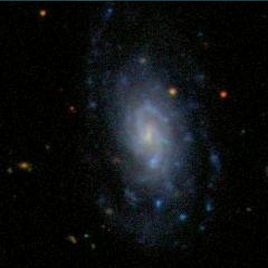
\includegraphics[scale=0.3]{UGC07012.png}
\caption{UGC07012}
\end{figure}
\begin{figure}
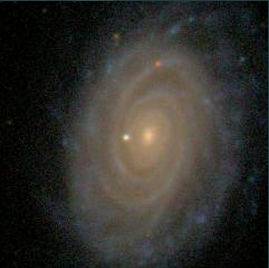
\includegraphics[scale=0.3]{NGC4185.png}
\caption{NGC4185}
\end{figure}
\begin{figure}
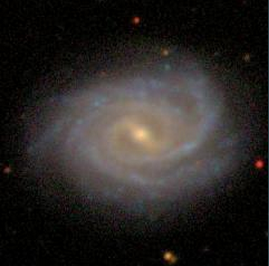
\includegraphics[scale=0.3]{NGC4210.png}
\caption{NGC4210}
\end{figure}
\begin{figure}
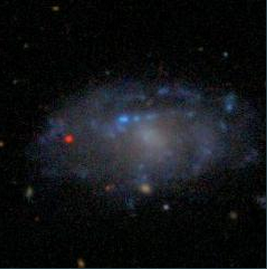
\includegraphics[scale=0.3]{IC0776.png}
\caption{IC0776}
\end{figure}
\begin{figure}
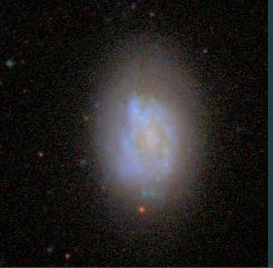
\includegraphics[scale=0.3]{NGC4470.png}
\caption{NGC4470}
\end{figure}

\clearpage

\begin{figure}
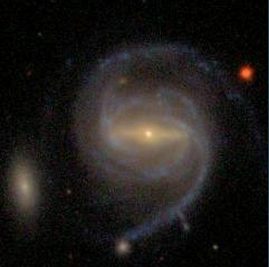
\includegraphics[scale=0.3]{NGC5000.png}
\caption{NGC5000}
\end{figure}
\begin{figure}
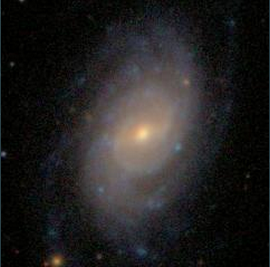
\includegraphics[scale=0.3]{NGC5205.png}
\caption{NGC5205}
\end{figure}
\begin{figure}
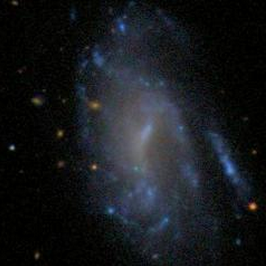
\includegraphics[scale=0.3]{UGC08733.png}
\caption{UGC08733}
\end{figure}
\begin{figure}
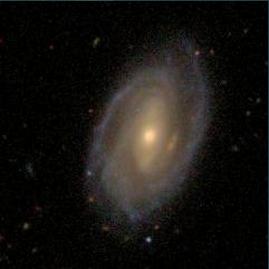
\includegraphics[scale=0.3]{UGC08781.png}
\caption{UGC08781}
\end{figure}
\begin{figure}
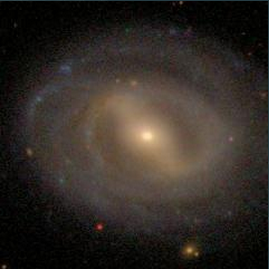
\includegraphics[scale=0.3]{NGC5378.png}
\caption{NGC5378}
\end{figure}

%\clearpage

\begin{figure}
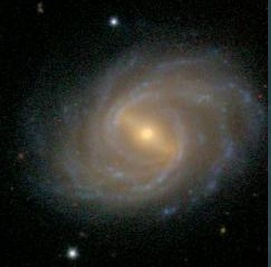
\includegraphics[scale=0.3]{NGC5406.png}
\caption{NGC5406}
\end{figure}
\begin{figure}
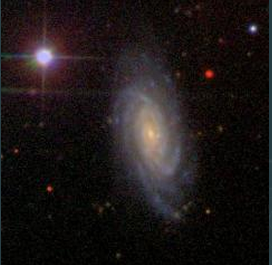
\includegraphics[scale=0.3]{UGC09067.png}
\caption{UGC09067}
\end{figure}
\begin{figure}
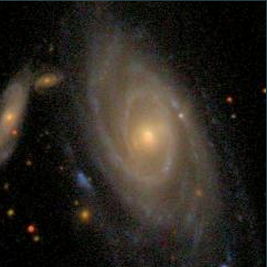
\includegraphics[scale=0.3]{NGC0036.png}
\caption{NGC0036}
\end{figure}
\begin{figure}
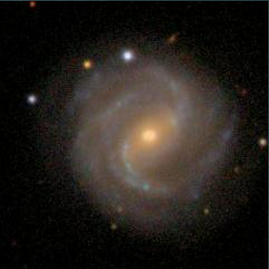
\includegraphics[scale=0.3]{NGC0776.png}
\caption{NGC0776}
\end{figure}
\begin{figure}
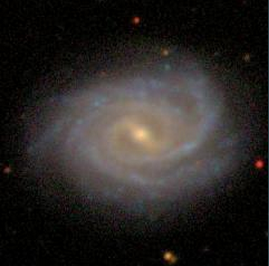
\includegraphics[scale=0.3]{NGC4210.png}
\caption{NGC4210}
\end{figure}

\clearpage

\begin{figure}
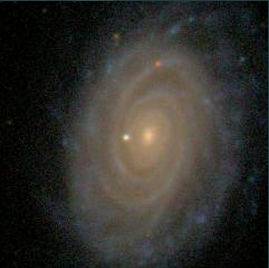
\includegraphics[scale=0.3]{NGC4185}
\caption{NGC4185}
\end{figure}
\begin{figure}
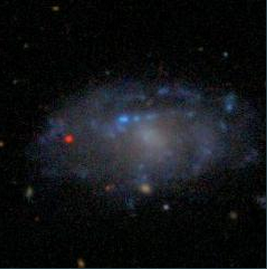
\includegraphics[scale=0.3]{IC0776.png}
\caption{IC0776}
\end{figure}
\begin{figure}
\includegraphics[scale=0.3]{NGC5000.png}
\caption{NGC5000}
\end{figure}
\begin{figure}
\includegraphics[scale=0.3]{UGC08781.png}
\caption{UGC08781}
\end{figure}
\begin{figure}
\includegraphics[scale=0.3]{NGC5406.png}
\caption{NGC5406}
\end{figure}

%\clearpage

\begin{figure}
\includegraphics[scale=0.3]{NGC5520.png}
\caption{NGC5520.png}
\end{figure}
\begin{figure}
\includegraphics[scale=0.3]{NGC5614.png}
\caption{NGC5614}
\end{figure}
\begin{figure}
\includegraphics[scale=0.3]{NGC5630.png}
\caption{NGC5630}
\end{figure}
\begin{figure}
\includegraphics[scale=0.3]{NGC5720.png}
\caption{NGC5720}
\end{figure}
\begin{figure}
\includegraphics[scale=0.3]{UGC09476.png}
\caption{UGC09476}
\end{figure}

\clearpage

\begin{figure}
\includegraphics[scale=0.3]{NGC5888.png}
\caption{NGC5888}
\end{figure}
\begin{figure}
\includegraphics[scale=0.3]{IC4566.png}
\caption{IC4566}
\end{figure}
\begin{figure}
\includegraphics[scale=0.3]{NGC6004.png}
\caption{NGC6004}
\end{figure}
\begin{figure}
\includegraphics[scale=0.3]{NGC6063.png}
\caption{NGC6063}
\end{figure}
\begin{figure}
\includegraphics[scale=0.3]{NGC6154.png}
\caption{NGC6154}
\end{figure}
\begin{figure}
\includegraphics[scale=0.3]{IC1256.png}
\caption{IC1256}
\end{figure}
\begin{figure}
\includegraphics[scale=0.3]{NGC6941.png}
\caption{NGC6941}
\end{figure}
\begin{figure}
\includegraphics[scale=0.3]{UGC11649.png}
\caption{UGC11649}
\end{figure}
\begin{figure}
\includegraphics[scale=0.3]{NGC7321.png}
\caption{NGC7321}
\end{figure}
\begin{figure}
\includegraphics[scale=0.3]{UGC12224.png}
\caption{UGC12224}
\end{figure}

\clearpage

\begin{figure}
\includegraphics[scale=0.3]{NGC7489.png}
\caption{NGC7489}
\end{figure}
\begin{figure}
\includegraphics[scale=0.3]{NGC7625.png}
\caption{NGC7625}
\end{figure}
\begin{figure}
\includegraphics[scale=0.3]{NGC7653.png}
\caption{NGC7653}
\end{figure}
\begin{figure}
\includegraphics[scale=0.3]{NGC7716.png}
\caption{NGC7716}
\end{figure}
\begin{figure}
\includegraphics[scale=0.3]{NGC5947.png}
\caption{NGC5947}
\end{figure}

\end{document}